\documentclass[crop,tikz]{standalone}

\usetikzlibrary{arrows}
\usetikzlibrary{decorations.pathreplacing}
\begin{document}
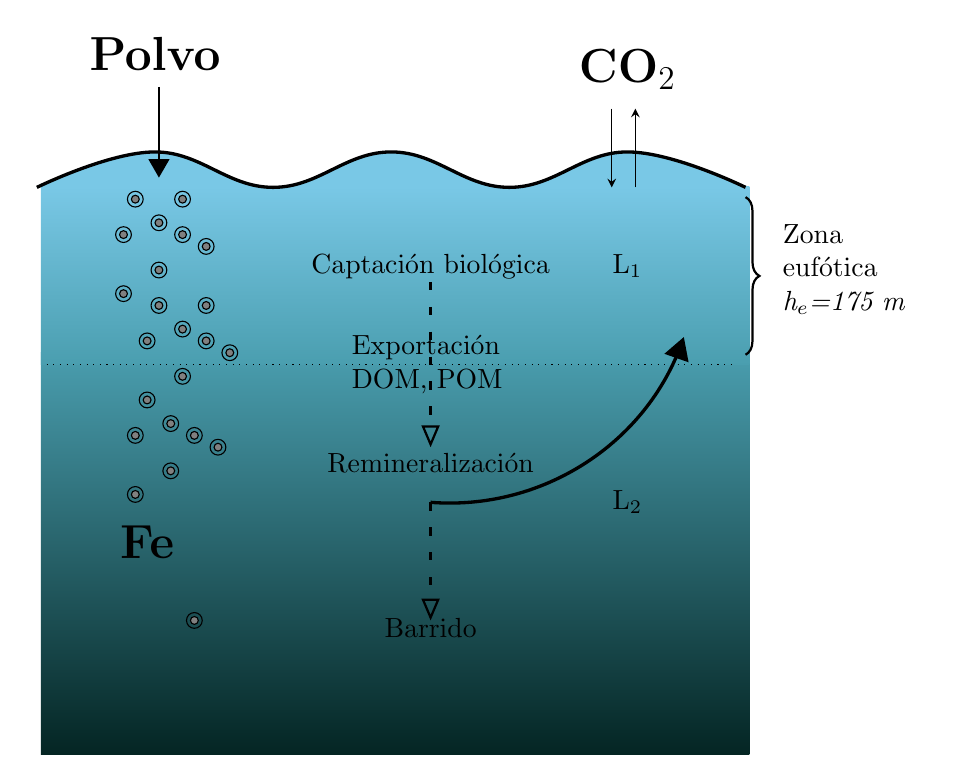
\begin{tikzpicture}
\shadedraw [draw=none, bottom color={rgb,255:red,4;green,37;blue,35},top color={rgb,255:red,74;green,158;blue,175}] (-4.95,-0.6) rectangle (4.05,-5.7);
\shadedraw [draw=none, bottom color={rgb,255:red,74;green,158;blue,175},top color={rgb,255:red,121;green,200;blue,230}] (-4.95,-0.75) rectangle (4.05,1.51);
%\draw [very thick] (-8.55,6.3) rectangle (6.9,-7.5); %BORRAR AL FINAL

\node at (0,0.5) {Captación biológica};

\node (v3) at (-5,1.5) {};
\node (v7) at (-2,1.5) {};
\node (v8) at (1,1.5) {};
\node (v4) at (4,1.5) {};


\node at (-3.5,3.2) {\LARGE{\bf Polvo}};

\node at (2.5,3) {\LARGE{\bf CO$_2$}};
\node at (0,-2) {Remineralización};

\node at (-3.6,-3) {\LARGE{\bf Fe}};
%\draw [double distance=2pt] (v3) edge (v4);
\node (v5) at (-5,-0.75) {};
\node (v6) at (4,-0.75) {};
\draw [dotted] (v5) edge (v6);

\draw [very thick,fill={rgb,255:red,121;green,200;blue,230}] plot[smooth, tension=.7] coordinates {(v3) (-3.5,1.95) (v7) (-0.5,1.95) (v8) (2.5,1.95) (v4)};

\node (v1) at (-3.45,2.9) {};
\node (v2) at (-3.45,1.5) {};

\draw [thick,-triangle 60] (v1) edge (v2);

\node[text width=2cm,] at (0,-0.75) {Exportación DOM, POM};
\draw [very thick,-triangle 60](-0.,-2.5) arc (-94.4321:-19.3125:3.15);

\draw [thick,decorate, decoration={brace, amplitude=5pt}](v4) -- (v6);
\node[text width=2cm,right] at (4.35,0.45) {Zona eufótica \textit{h$_e$=175 m}};

\draw  (-3.15,0.9) ellipse (0.1 and 0.1);
\draw[fill=gray]  (-3.15,0.9) ellipse (0.05 and 0.05);

\draw  (-3.9,0.9) ellipse (0.1 and 0.1);
\draw[fill=gray]  (-3.9,0.9) ellipse (0.05 and 0.05);

\draw  (-2.85,0.75) ellipse (0.1 and 0.1);
\draw[fill=gray]  (-2.85,0.75) ellipse (0.05 and 0.05);

\draw  (-3.15,1.35) ellipse (0.1 and 0.1);
\draw[fill=gray]  (-3.15,1.35) ellipse (0.05 and 0.05);

\draw  (-3.45,0.45) ellipse (0.1 and 0.1);
\draw[fill=gray]  (-3.45,0.45) ellipse (0.05 and 0.05);

\draw  (-3.9,0.15) ellipse (0.1 and 0.1);
\draw[fill=gray]  (-3.9,0.15) ellipse (0.05 and 0.05);

\draw  (-3.75,1.35) ellipse (0.1 and 0.1);
\draw[fill=gray]  (-3.75,1.35) ellipse (0.05 and 0.05);

\draw  (-3.45,1.05) ellipse (0.1 and 0.1);
\draw[fill=gray]  (-3.45,1.05) ellipse (0.05 and 0.05);

\draw  (-2.85,0) ellipse (0.1 and 0.1);
\draw[fill=gray]  (-2.85,0) ellipse (0.05 and 0.05);

\draw  (-3.45,0) ellipse (0.1 and 0.1);
\draw[fill=gray]  (-3.45,0) ellipse (0.05 and 0.05);

\draw  (-3.15,-0.3) ellipse (0.1 and 0.1);
\draw[fill=gray]  (-3.15,-0.3) ellipse (0.05 and 0.05);

\draw  (-3.6,-0.45) ellipse (0.1 and 0.1);
\draw[fill=gray]  (-3.6,-0.45) ellipse (0.05 and 0.05);

\draw  (-2.85,-0.45) ellipse (0.1 and 0.1);
\draw[fill=gray]  (-2.85,-0.45) ellipse (0.05 and 0.05);

\draw  (-2.55,-0.6) ellipse (0.1 and 0.1);
\draw[fill=gray]  (-2.55,-0.6) ellipse (0.05 and 0.05);

\draw  (-3.15,-0.9) ellipse (0.1 and 0.1);
\draw[fill=gray]  (-3.15,-0.9) ellipse (0.05 and 0.05);

\draw  (-3.6,-1.2) ellipse (0.1 and 0.1);
\draw[fill=gray]  (-3.6,-1.2) ellipse (0.05 and 0.05);


%%%

\draw  (-3.3,-1.5) ellipse (0.1 and 0.1);
\draw[fill=gray]  (-3.3,-1.5) ellipse (0.05 and 0.05);

\draw  (-3.75,-1.65) ellipse (0.1 and 0.1);
\draw[fill=gray]  (-3.75,-1.65) ellipse (0.05 and 0.05);

\draw  (-3,-1.65) ellipse (0.1 and 0.1);
\draw[fill=gray]  (-3,-1.65) ellipse (0.05 and 0.05);

\draw  (-2.7,-1.8) ellipse (0.1 and 0.1);
\draw[fill=gray]  (-2.7,-1.8) ellipse (0.05 and 0.05);

\draw  (-3.3,-2.1) ellipse (0.1 and 0.1);
\draw[fill=gray]  (-3.3,-2.1) ellipse (0.05 and 0.05);

\draw  (-3.75,-2.4) ellipse (0.1 and 0.1);
\draw[fill=gray]  (-3.75,-2.4) ellipse (0.05 and 0.05);

\draw  (-3,-4) ellipse (0.1 and 0.1);
\draw[fill=gray]  (-3,-4) ellipse (0.05 and 0.05);


\draw[thick,loosely dashed,-open triangle 45] (0,0.3) -- (0,-1.8);

\node at (2.5,0.5) {L$_1$};
\node at (2.5,-2.5) {L$_2$};
\draw [-stealth](2.3,2.5) -- (2.3,1.5);
\draw [-stealth](2.6,1.5) -- (2.6,2.5);
\node at (0,-4.1) {Barrido};
\draw[thick,loosely dashed] [-open triangle 45](0,-2.5) -- (0,-4);
\end{tikzpicture}

\end{document}
